\chapter{Consept\label{cha:chapter3}}
This section determines the requirements and design choices necessary for developing the RDF Instance Generator Schema Visualizer and the RDF web service.

\section{Overview\label{sec:reqoverview}}

This project aims to simplify RDF schema exploration, validation, and instance generation. To achieve this the following requirements are defined: 
\begin{itemize}
    \item Functional requirements, for core features like, instance generation, schema validation, and visualization.
    \item Non-functional requirements, to take into account performance, usability and compatibility.
    \item Technical requirements, specified for underlying technologies and system design.
    \item Data privacy and Security, useful to ensure the security and privacy of user data.
\end{itemize}

The design prioritizes a client-server architecture, and cross-platform compatibility to enhance usability and efficiency. 
\\
The Web Service is designed to be compatible with various Browsers and IDEs. 
\\
The IDE extension will support users and will seamlessly integrate in their workflow.
\section{Functional requirements\label{sec:techreq}}
In this section covers the functional requirements for the entire system.

\subsection{Instance Generation\label{sec:reqsuba}}
The very first requirement for this project is the generation of synthetic RDF instances.
\\
When the user is writing an RDF file, in turtle, N3, XML or other RDF formats, it will generate some synthetic RDF instances that could save him a lot of time avoiding the insertion of testing data.
\\
The application will not just generate compatible triples instances, but also allow the user to modify the automatically generated instances.

\subsection{Schema Validation\label{sec:reqsuba}}
The Program should be designed to validate a user-defined RDF schema by checking the structural integrity and semantic consistency of its triples. 
Each triple conforms to syntactic constraints (e.g., proper use of IRIs, literals, and blank nodes) and the asserted relationships lead to any logical contradictions or unexpected inferences.
\\
In case of errors in the schema description, feedback should be provided to the user, via UI or Terminal.

\subsection{Multi-Vocabulary Support\label{sec:reqsuba}}
Interoperability and semantic richness are crucial for ensuring seamless data integration, enhancing knowledge representation, and enabling efficient querying and reasoning across diverse RDF datasets.
By supporting multiple vocabularies and ontologies such as RDFS, FOAF, Schema.org and others, the system should be able to handle a wide range of RDF data sources and their visualization as graphs.

\subsection{Import and Export\label{sec:reqsuba}}
The software should allow the users to import their custom RDF files, and export the file with the automatic generated instances in the same format.

\subsection{Schema Visualization\label{sec:reqsuba}}
To simplify the exploration and analyzes of an RDF from a human eye, the program should be able to display the described RDF schema with its graphical representation.
The displayed graph should have some interactive features like zooming, panning and node collapse.
\\
The graphical representation should adapt based on the schema complexity and hierarchical structure.
\\
In the IDE  extension, the user should be able to visualize the graph in a side panel window next to the RDF file their working on. 

\section{Non-functional requirements\label{sec:techreq}}
This section determines the non-functional requirements of the system.

\subsection{Performance\label{sec:reqsuba}}
The system should ensure high performance rendering of large RDF graphs to facilitate seamless visualization and interaction. Additionally, operations such as node selection and zooming should be executed with minimal latency to maintain a responsive user experience. The system should optimize rendering pipelines to support real-time exploration of complex RDF schemas without compromising efficiency.

\subsection{Usability\label{sec:reqsuba}}
Both the IDE extension and the web application should feature an intuitive and user-centric interface that enhances accessibility and minimizes the learning curve for users. To achieve this objective, the design should incorporate familiar UI elements or skeuomorphic design principles, ensuring a seamless and intuitive user experience. 

\subsection{Compatibility\label{sec:reqsuba}}
To ensure seamless integration across various development environments, the web service should be designed with cross-platform compatibility, enabling effortless adoption in different IDEs with minimal modifications. This approach enhances interoperability, allowing the service to function efficiently within diverse software ecosystems while maintaining consistent performance and usability. 
\\
To validate this, minor features in a secondary IDE should be implemented.


\section{Technical Requirements\label{sec:techreq}}

\subsection{Web Architecture\label{sec:reqsuba}}
The system should be designed with a client-server architecture. There are no constraints on the specific technologies (e.g. SOAP, REST, gRPC), but it must follow the web principles and use Web technologies, such as HTML, CSS, JavaScript or WebAssembly, and protocols (e.g. HTTP, WebSockets).

\subsection{IDE extension\label{sec:reqsuba}}
The application should be accessible via a web-based client to ensure broad availability; however, primary emphasis should be placed on its integration as an extension within widely used IDEs. 

\section{Data privacy and Security\label{sec:techreq}}
\subsection{Security\label{sec:reqsuba}}
To ensure the confidentiality and integrity of RDF data, the system should implement secure data transmission protocols, such as HTTPS, to protect sensitive information during transmission.

\subsection{Confidentiality\label{sec:reqsuba}}
Based on the current design, no information should be saved from the Business Logic Layer. 
\\
All data processing occurs in-memory, either on the client-side or server-side, ensuring that no persistent storage of user data takes place within the system. This ephemeral data handling approach significantly reduces the risk of data retention and unauthorized access. As a result, compliance requirements related to long-term data storage, such as those outlined in the General Data Protection Regulation (GDPR), are minimized. 


\section{Solution strategy\label{sec:techreq}}
As stated previously in the requirements section, the system is designed with a client-server architecture, where the client and server play distinct roles in the overall functionality.

\begin{figure}[H]
    \centering
    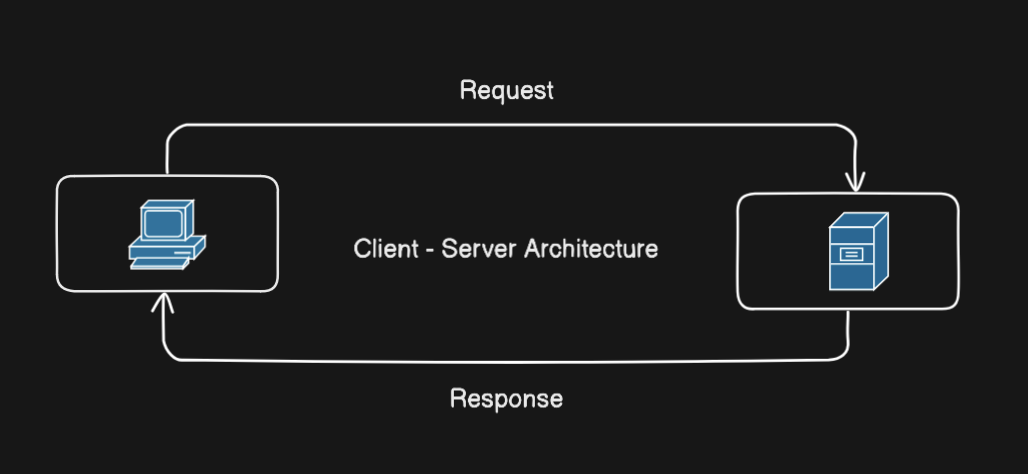
\includegraphics[width=14cm]{client_server.png}\\
    \caption{Client / Server}\label{fig:client_server}
  \end{figure}

\subsection{Client\label{sec:reqsuba}}
To ensure a broad availability of the system, the system is designed to support two type of user-agents:
\begin{itemize}
    \item Browsers
    \item Integrated Development Environments 
\end{itemize}
The Browser chosen by the user, should be able to access the web application via HTTP requests protocol.
The user will then upload their RDF file and send it to the server.
The Client will then receive the processed information and display the resulting graph (see Figure \ref{fig:BrowserGraphView}).

\begin{figure}[htb]
    \centering
    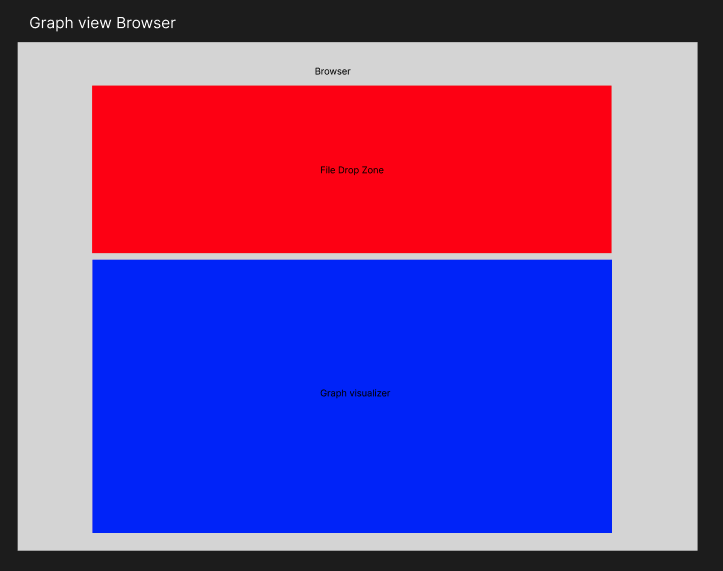
\includegraphics[width=14cm]{mock dropzone.png}\\
    \caption{Browser file drop zone and graph view }\label{fig:BrowserGraphView}
  \end{figure}

In addition to this, the user should be able to read the RDF file with the generated instances next to its graphical representation (see Figure \ref{fig:BrowserRDFReader}).

\begin{figure}[htb]
    \centering
    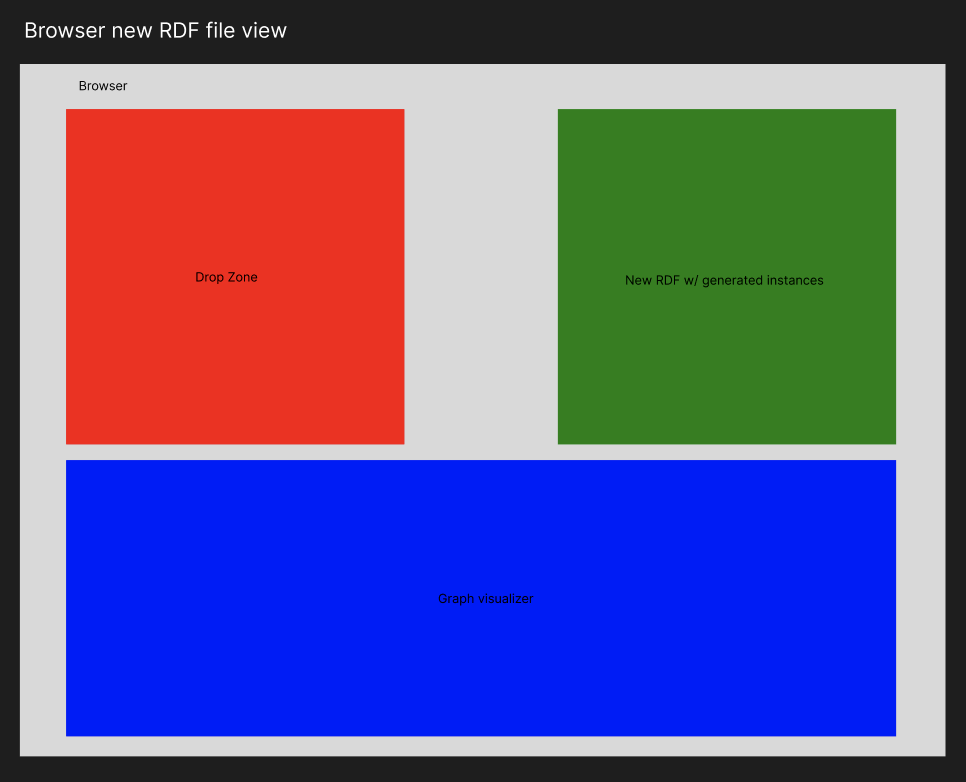
\includegraphics[width=14cm]{mock_browser_new_RDF_instance.png}\\
    \caption{Browser new RDF side panel view }\label{fig:BrowserRDFReader}
  \end{figure}

Within the IDE, the user experience UX will be slight different from the Browser one. Instead of manually uploading an RDF file, users will interact with the system directly within the IDE. By working on an RDF file and executing a predefined command, a web-based visualization panel of the file on focus will be dynamically launched as a side panel within the IDE. This panel will render an interactive graphical representation of the RDF schema in real time, allowing users to analyze relationships, structures, and dependencies without disrupting their coding environment (see Figure \ref{fig:IDEGraphView}). 

\begin{figure}[H]
    \centering
    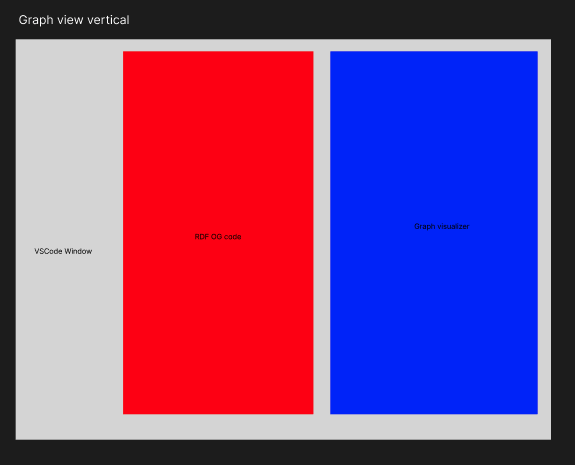
\includegraphics[width=14cm]{mockup side panel view.png}\\
    \caption{IDE Graph side panel view}\label{fig:IDEGraphView}
  \end{figure}

  The extension will not only support the visualization of RDF files in the format requested by the user, similar to its browser counterpart, but it will also enable real-time modification of the file (see Figure \ref{fig:IDERDFReader}).

  \begin{figure}[htb]
      \centering
      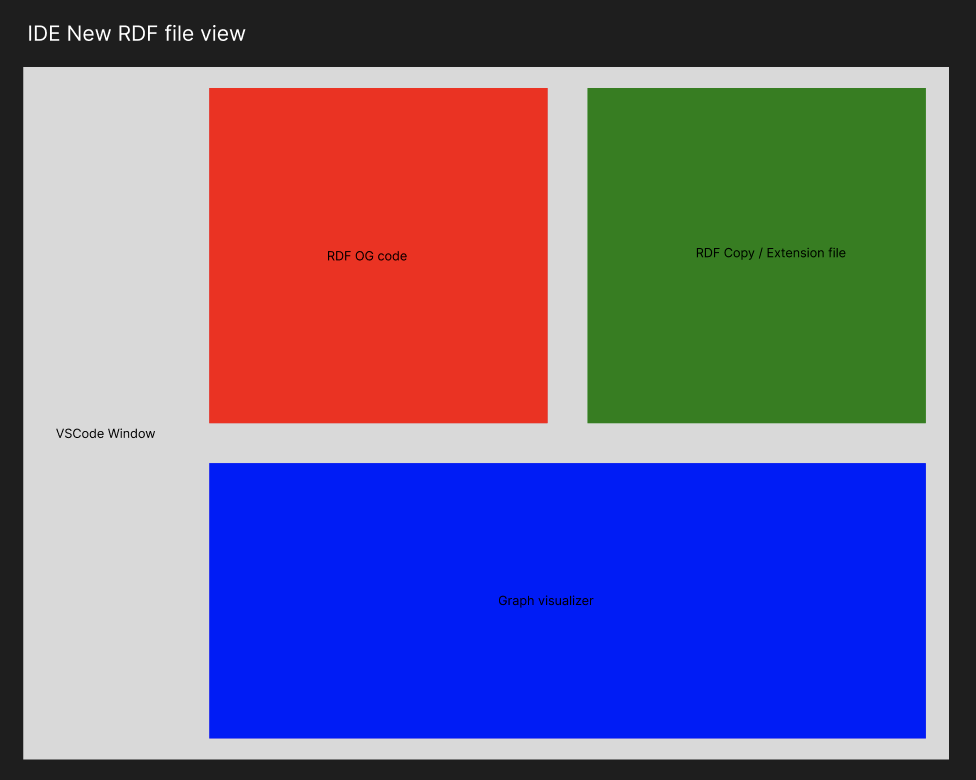
\includegraphics[width=14cm]{mock_ide_new_RDF_instance.png}\\
      \caption{IDE new RDF side panel view}\label{fig:IDERDFReader}
    \end{figure}

  \subsection{Server\label{sec:server}}
  To assure system intercompatibility across various device, Operative Systems, and User-Agents, the server is responsible for all computational tasks and data processing. By centralizing calculations and graph data manipulation on the server side, the server minimizes client-side resource consumption and enhances performance consistency. 
  \\
  \\
  The server place a crucial role in managing RDF data ensuring  schema validation, instance generation, SPARQL query processing, and graph construction.
  \\
  When the server receives an RDF file, it must scan the file to see potential floss, syntactic or semantic errors. It should be able to handle multiple RDF serialization formats such as Turtle, N3, XML, and JSON-LD. 
  \\
  \\
  The service generates synthetic RDF instances based on a given schema. It ensures logical consistency between the generated schema and the original one.
  \\
  The system identifies classes and properties within an RDF schema and generates additional instances, where necessary, to maintain semantic correctness. 
  \\
  This is particularly important in cases where a property references an instance of a specific class that has not been explicitly defined in the dataset.
  For example, if a schema includes a hasCar property that requires an instance of the Car class, but no such instance exists, the system should automatically create one. This ensures that the schema remains logically consistent and that all property constraints are met. By dynamically generating required instances, the system helps maintain data integrity, prevents incomplete assertions, and improves the reliability of reasoning processes within RDF applications.
  \\ 
  The additional generated instances have realistic properties and values in order to fulfill the graph constraints.
  \\
  \\
  The service serves the new RDF file in the requested format with its graphical representation.